\Chapter{A játék matematikai modellje}


\begin{figure}[h]
\centering
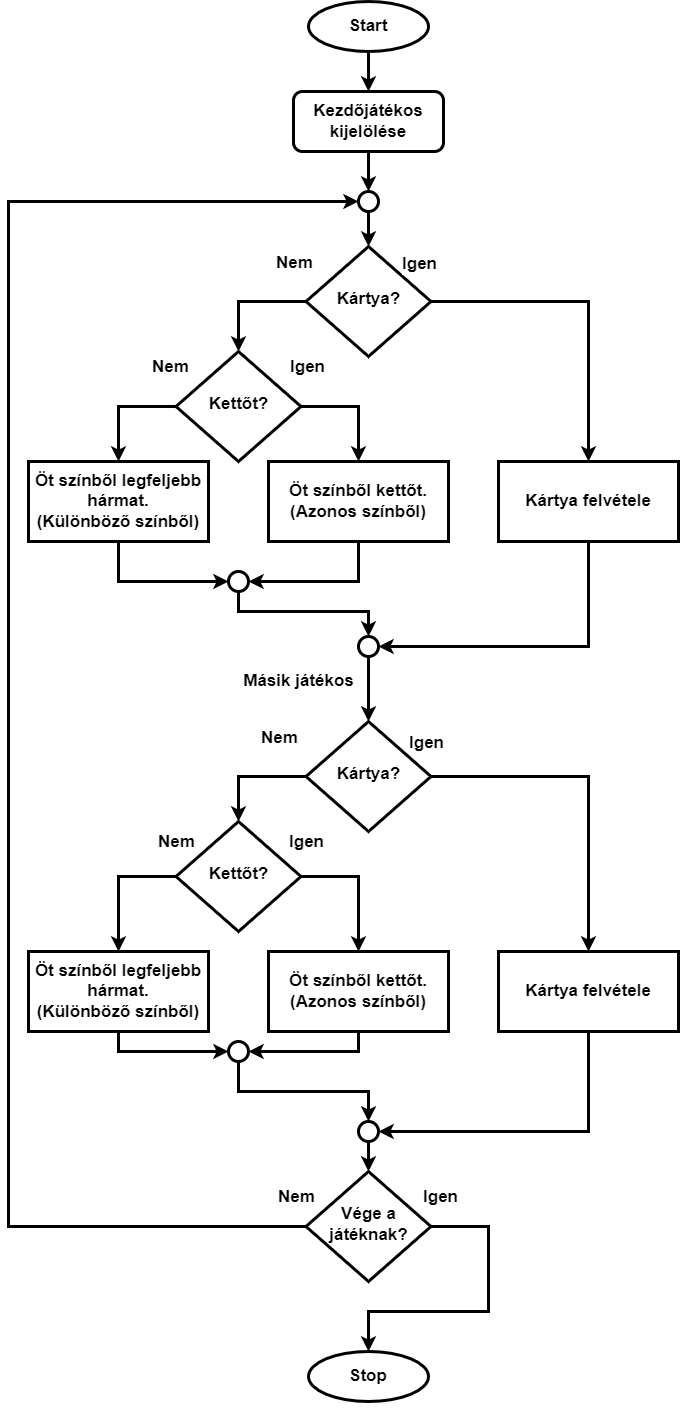
\includegraphics[scale=0.3]{images/flowchart.png}
\caption{A játék folyamatábrája.}
\label{fig:flowchart}
\end{figure}


Ahogy folyamatábrán is látható a játék köreinek felépítése viszonylag egyszerűen zajlik. Kezdetben kijelöljük a éppen soron lévő játékost, majd megkezdődik a köre. Először eldönti, hogy kártyát vagy zsetont szeretne választani. Ha kártyát, akkor a kártyahúzás után vége a körének. Ha viszont zsetont, akkor két lehetőség áll a rendelkezésére. Vagy hármat választ, egyet-egyet a különböző színekből, vagy pedig kettőt, de azonos színből. A két lehetőség valamelyikének végrehajtása után szintén véget ér a kör. Ezután megvizsgáljuk, hogy megvalósult-e a játék végét jelentő feltétel. Ha nem, akkor a folyamat elejére ugorva kiválasztjuk a másik játékost és megkezdődik a köre, amiben ugyanezekkel a lehetőségekkel rendelkezik. Ha pedig igen, akkor a játék befejeződik.

A játékos természetesen csak a számára elérhető kártyákból és zsetonokból választhat. Egy zseton akkor elérhető a számára, ha abból legalább egy van a játéktéren, a kártya pedig akkor, ha a megvásárlásához szükséges zsetonok a birtokában vannak. Ezek a zsetonok lehetnek sima, korábban elvett zsetonok, vagy akár a kártyák korábbi megvásárlása nyomán megszerzett bónusz értékek.

A kártyalapok a játéktérre való elhelyezése randomizlálva történik az adott szintű kártyapaklikból megfelelően. A kártyák szimmetrikusan szerepelnek a paklikban, így ezek teljesen egyenértékűek a teljes kártyakészletre nézve. A játék előrehaladtával és a kártyalapok és zsetonok fogyásával értelemszerűen folyamatosan változik az adott játékos számára elérhető lehetőségeknek az értéke. Ezeket az értékeket különféle preferenciák alapján lehet meghatározni, mivel minden játékos az adott stílusában játszik. Lehet a lehető legmagasabb pontszámú kártyákra, lehet több kisebb értékű lapra gyűjteni. Lehet a játékos saját bónuszait figyelve megfelelően felépíteni egy jól működő mechanizmust, viszont lehet az ellenfél lépését megakadályozó taktikát is követni. Ezáltal nincsen rendszer, ami alapján pontosan meg tudjuk meghatározni, hogy egy adott játékállapotban az adott játékos számára mi a lehető legmegfelelőbb lépés.

